% !TeX root = ../thuthesis-example.tex

\chapter{神经网络中的李雅普诺夫谱}

\section{符号约定}

在分析神经网络的李雅普诺夫谱时,我们使用以下符号约定,如表 \ref{tab:symbols} 所示.

\begin{table}[htbp]
  \centering
  \caption{符号约定}
  \label{tab:symbols}
  \begin{tabular}{cc}
    \toprule
    符号                      & 含义                                             \\
    \midrule
    \(x_l\)                   & 第 \(l\) 层的状态向量                            \\
    \(\mathbf{J}_l\)          & 第 \(l\) 层的雅可比矩阵                          \\
    \(\mathbf{R}_l\)          & 第 \(l\) 层的上三角矩阵                          \\
    \(\mathbf{Q}_l\)          & 第 \(l\) 层的正交矩阵                            \\
    \(\lambda_{forward, i}\)  & 正向传播的第 \(i\) 个李雅普诺夫指数              \\
    \(\lambda_{backward, i}\) & 反向传播的第 \(i\) 个李雅普诺夫指数              \\
    \(q_{ij}^{+}\)             & 正向传播中第 \(i\) 层的第 \(j\) 个偏置向量 \\
    \(q_{ij}^{-}\)      & 反向传播中第 \(i\) 层的第 \(j\) 个偏置向量 \\
    \bottomrule
  \end{tabular}
\end{table}

\section{理论分析}

伴随李雅普诺夫谱是指在系统反向传播过程中计算得到的李雅普诺夫指数。理论上,正向传播和反向传播的李雅普诺夫谱应该具有一定的对偶性,即相同方向对应的正向和反向传播的两个向量内积不随时间变化.
\begin{equation}
  \langle q_{i j}^{+}, q_{i j}^{-} \rangle = \text{常数}.
\end{equation}

\subsection{研究方案}

为了验证这一结论,本文进行了以下研究:

\begin{enumerate}
  \item 正向传播计算:按照前述步骤,计算神经网络在正向传播过程中的李雅普诺夫谱 \(\lambda_{forward, i}\).
  \item 反向传播计算:在反向传播过程中,同样计算出相应的李雅普诺夫谱 \(\lambda_{backward, i}\).
  \item 对偶性验证:计算正向和反向的李雅普诺夫谱的同时,会得到每一步的中间向量 \(q_{ij}^{+}\) 和 \(q_{ij}^{-}\). 我们发现这两个向量具有“对偶性”。
\end{enumerate}

\subsection{对偶性的定义及理论证明}

设正向传播中第 \(i\) 层的第 \(j\) 个中间向量为 \(q_{ij}^{+}\),反向传播中第 \(i\) 层的第 \(j\) 个中间向量为 \(q_{ij}^{-}\),则对偶性定义为:
\begin{equation}\label{eq:duality}
  \langle q_{ij}^{+}, q_{ij}^{-} \rangle = \text{常数}.
\end{equation}

证明如下:
\begin{equation}
  \begin{aligned}
    \langle q_{ij}^{+}, q_{ij}^{-} \rangle & = (J^T \cdot q_{ij}^{-})^T\cdot {q_{ij}^{+}}^T \\
                                            & = {q_{ij}^{-}}^T \cdot (J \cdot q_{ij}^{+})    \\
                                            & = {q_{ij}^{-}}^T \cdot q_{ij+1}^{+}            \\
                                            & = \langle q_{ij+1}^{+}, q_{ij+1}^{-} \rangle.
    \end{aligned}
\end{equation}

我们将在 \ref{sec:duality} 一节验证这一现象,但下一节将首先介绍前述算法在全连接神经网络中和循环神经网络中的应用。

\section{实验分析}

本章的最终目的在于使用算法 \ref{alg:lyapunov} 验证 \ref{eq:duality},首先展示该算法在全连接神经网络中的表现:

\subsection{全连接神经网络}

\subsubsection{网络结构}

选取一个三层全连接神经网络,针对 $28\times 28$ 的灰度图像数据集(例如 MNIST 手写数字数据集)进行训练。网络参数和结构示意图如下所示:

\begin{enumerate}
  \item 输入层:维度为 28x28=784.
  \item 隐藏层:一个,维度为 50,激活函数为 ReLU.
  \item 输出层:维度为 10,激活函数为 Softmax.
\end{enumerate}

\begin{figure}[htbp]
  \centering
  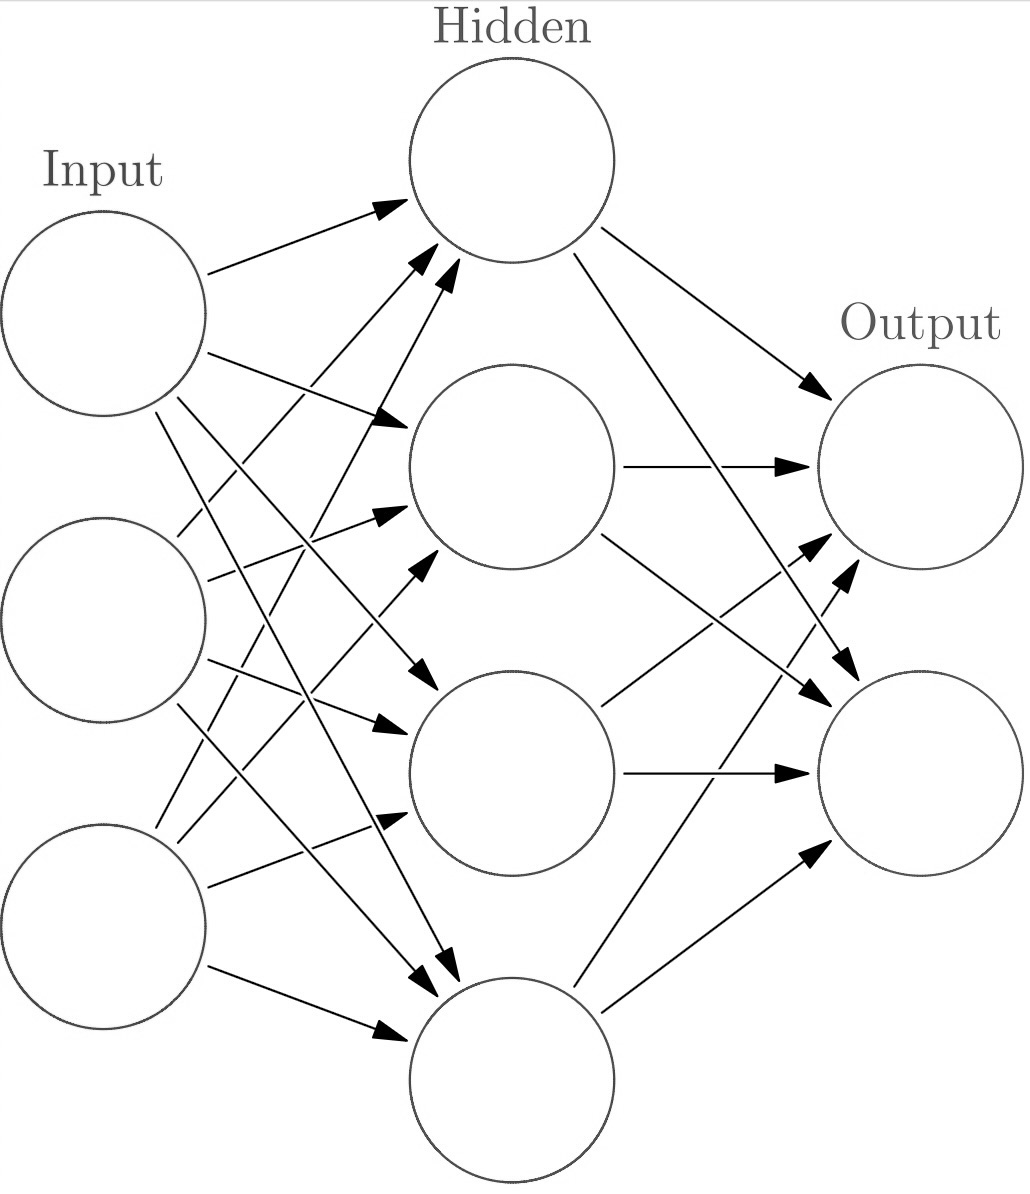
\includegraphics[width=0.5\textwidth]{figures/nn.jpeg}
  \caption{全连接神经网络}
  \label{fig:example}
\end{figure}

首先,我们选定网络每层的初始状态:

\begin{enumerate}
  \item 输入层:接受 $28\times28$ 的灰度图像作为输入,展平成784维的向量:
        \begin{equation}
          \mathbf{x} \in \mathbb{R}^{784}.
        \end{equation}

  \item 隐藏层:一个全连接层,包含50个神经元,激活函数为ReLU:
        \begin{equation}
          \mathbf{h} = \text{ReLU}(\mathbf{W}_1 \mathbf{x} + \mathbf{b}_1).
        \end{equation}
        其中,\(\mathbf{W}_1 \in \mathbb{R}^{50 \times 784}\) 为权重矩阵,\(\mathbf{b}_1 \in \mathbb{R}^{50}\) 为偏置向量。

  \item 输出层:一个全连接层,包含10个神经元,激活函数为Softmax:
        \begin{equation}
          \mathbf{y} = \text{Softmax}(\mathbf{W}_2 \mathbf{h} + \mathbf{b}_2).
        \end{equation}
        其中,\(\mathbf{W}_2 \in \mathbb{R}^{10 \times 50}\) 为权重矩阵,\(\mathbf{b}_2 \in \mathbb{R}^{10}\) 为偏置向量。
\end{enumerate}

约定这个神经网络中的符号如下表所示:

\begin{table}[htbp]
  \centering
  \caption{神经网络参数符号}
  \label{tab:nn}
  \begin{tabular}{cc}
    \toprule
    符号             & 含义           \\
    \midrule
    \(\mathbf{x}\)   & 输入向量       \\
    \(\mathbf{h}\)   & 隐藏层输出     \\
    \(\mathbf{y}\)   & 输出层输出     \\
    \(\mathbf{W}_1\) & 隐藏层权重矩阵 \\
    \(\mathbf{b}_1\) & 隐藏层偏置向量 \\
    \(\mathbf{W}_2\) & 输出层权重矩阵 \\
    \(\mathbf{b}_2\) & 输出层偏置向量 \\
    \bottomrule
  \end{tabular}
\end{table}

\subsubsection{训练过程}

训练该神经网络用到 60000 组学习数据和 10000 组测试数据,这些数据从 MNIST 数据集中导入,满足归一化条件,即 784 个像素的灰度值均用 $[0, 1]$ 区间内的实数表示。

令总迭代次数为 10000 次,每个 batch 包含 100 组学习数据,设定学习率为 0.1,然后开始训练。下图展示了训练过程中神经网络的准确率变化。

\begin{figure}[htbp]
  \centering
  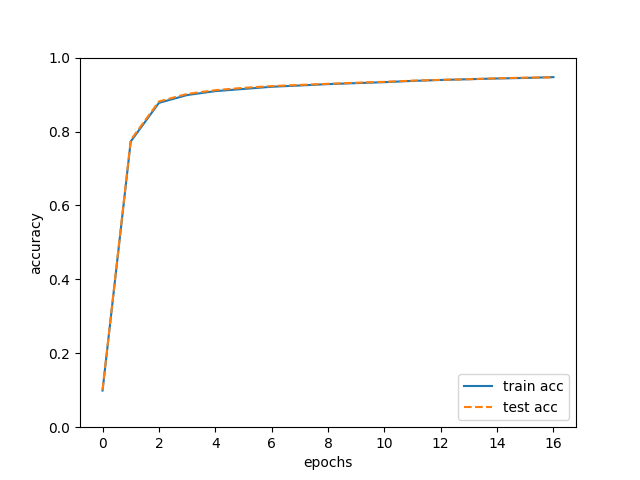
\includegraphics[width=1\textwidth]{figures/output.png}
  \caption{准确率变化折线图}
  \label{fig:nn_lyapunov_exponents}
\end{figure}

训练完成后,保存所有参数并在下一节中使用。

\subsubsection{李雅普诺夫谱计算}

读取上一节保存的参数,使神经网络恢复到训练完成的状态。随机选取输入值 $x$ 和随机梯度,得到确定的状态 $x$、$h$、$y$ 和梯度 $\frac{\partial y}{\partial h}$、$\frac{\partial h}{\partial x}$.

矩阵 $Q_0$ 为随机矩阵 QR 分解后的结果,记 $v_0 = Q_0$,其含义为 10 个不同方向的输入层向量。

正向传播:

\begin{equation}
  \left\{
    \begin{aligned}
      v_1 &= \frac{\partial h}{\partial x} v_0 \\
      v_2 &= \frac{\partial y}{\partial h} v_1
    \end{aligned}
  \right.
\end{equation}

反向传播:

\begin{equation}
  \left\{
    \begin{aligned}
      \nu_1 &= \frac{\partial h}{\partial x} \nu_2 \\
      \nu_0 &= \frac{\partial y}{\partial h} \nu_1
    \end{aligned}
  \right.
\end{equation}

计算正向和反向传播的同时,使用算法 \ref{alg:lyapunov} 计算 $v$ 和 $\nu$ 的李雅普诺夫谱。

全连接神经网络不能随时间无限延伸,正向和反向的传播均只进行两步,但可以通过多组输入来发现一般规律。

尝试 20 组不同的 $x$ 输入,得到 20 组不同的李雅普诺夫谱,每组有 10 个指数,总体上呈现下降趋势:

\begin{figure}[htbp]
  \centering
  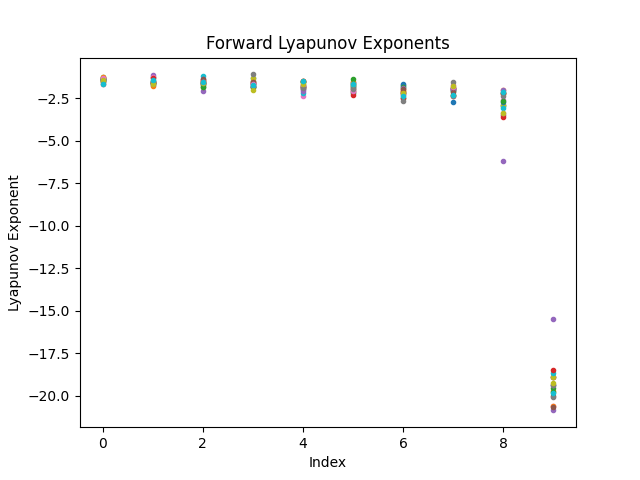
\includegraphics[width=1\textwidth]{figures/forward_lyapunov.png}
  \caption{正向传播的李雅普诺夫指数}
  \label{fig:nn_lyapunov_exponents}
\end{figure}

\begin{figure}[htbp]
  \centering
  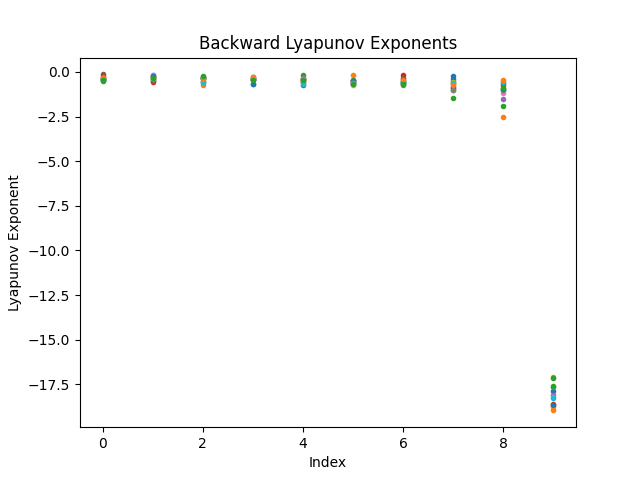
\includegraphics[width=1\textwidth]{figures/backward_lyapunov.png}
  \caption{反向传播的李雅普诺夫指数}
  \label{fig:nn_lyapunov_exponents}
\end{figure}

将多组数据取平均,得到如下散点图:

\begin{figure}[htbp]
  \centering
  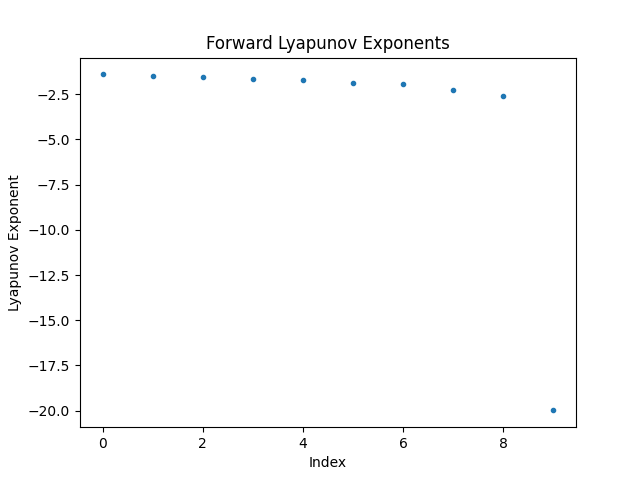
\includegraphics[width=1\textwidth]{figures/forward_lyapunov_avg.png}
  \caption{正向传播的平均李雅普诺夫指数}
  \label{fig:nn_lyapunov_exponents}
\end{figure}

\begin{figure}[htbp]
  \centering
  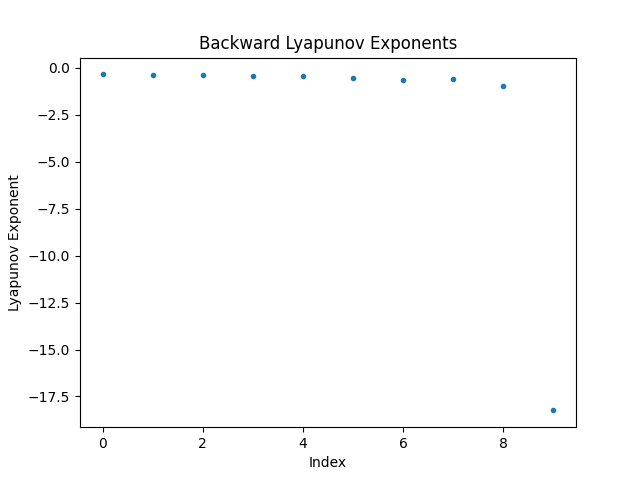
\includegraphics[width=1\textwidth]{figures/backward_lyapunov_avg.png}
  \caption{反向传播的平均李雅普诺夫指数}
  \label{fig:nn_lyapunov_exponents}
\end{figure}

\subsubsection{结果分析}

李雅普诺夫指数的个数由节点数目最少的输出层决定,在该网络中为 10 个。由上一小节的散点图,可以发现如下规律:

\begin{enumerate}
  \item 10 个李雅普诺夫指数均小于 0,说明该神经网络代表的动力系统是稳定的,不会出现梯度爆炸。
  \item 绝大多数方向的李雅普诺夫指数接近 0,意味着一般情况下,神经网络的梯度不会发生显著的梯度消失。
  \item $x=9$ 上的李雅普诺夫指数明显远小于其他方向,在这个方向上的梯度可能出现明显的梯度消失。
\end{enumerate}

至此已经完成了算法 \ref{alg:lyapunov} 的运行,但考虑到该全连接神经网络中间层的维数偏多,若验证对偶性将花费过长时间,因此我们将在下一节中考虑隐藏层维数较小的循环神经网络(RNN)。

\clearpage

\subsection{循环神经网络}\label{sec:rnn}

\subsubsection{网络结构}

RNN 在处理序列数据方面具有显著优势,能够捕捉时间步长上的依赖关系。在本实验中,我们选取一个循环神经网络(RNN),分别针对无输入、有输入的情形进行计算。选取任意时间步长 $T$,如下图示设计了一个简单的 RNN 模型,然后使用李雅普诺夫谱分析其动态行为。

和全连接神经网络类似,我们先尝试运行算法 \ref{alg:lyapunov},首先确定神经网络的参数规模和结构:

\begin{enumerate}
  \item 输入层:每个时间步的输入维度为 2
  \item 隐藏层:一个,隐藏状态维度为 3,激活函数为 tanh
  \item 输出层:维度为 2,激活函数为 Softmax
\end{enumerate}

\begin{figure}[htbp]
  \centering
  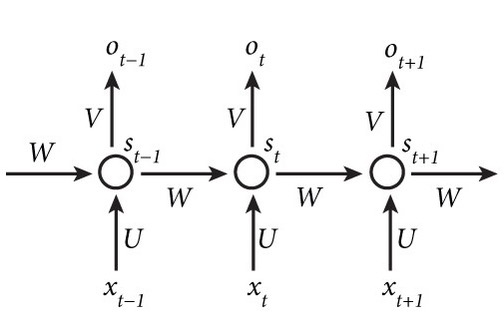
\includegraphics[width=0.5\textwidth]{figures/rnn.jpeg}
  \caption{循环神经网络}
  \label{fig:example}
\end{figure}

其次确定激活函数、权重矩阵和偏置向量:

\begin{enumerate}

  \item 输入层:每个时间步的输入维度为 2,时间步可任意长(在程序可计算的范围内)
        \begin{equation}
          \mathbf{x}_t \in \mathbb{R}^{3}.
        \end{equation}

  \item 隐藏层:一个 RNN 层,隐藏状态维度为 3,激活函数为 tanh:
        \begin{equation}
          \mathbf{h}_t = \text{tanh}(\mathbf{W}_{hh} \mathbf{h}_{t-1} + \mathbf{W}_{xh} \mathbf{x}_t + \mathbf{b}_h).
        \end{equation}
        其中,\(\mathbf{W}_{hh} \in \mathbb{R}^{3 \times 3}\) 和 \(\mathbf{W}_{xh} \in \mathbb{R}^{3 \times 3}\) 分别为隐藏状态和输入的权重矩阵,\(\mathbf{b}_h \in \mathbb{R}^{3}\) 为偏置向量。

  \item 输出层:维度为 3,激活函数为 Softmax:
        \begin{equation}
          \mathbf{y}_t = \text{Softmax}(\mathbf{W}_{hy} \mathbf{h}_t + \mathbf{b}_y).
        \end{equation}
        其中,\(\mathbf{W}_{hy} \in \mathbb{R}^{3 \times 3}\) 为权重矩阵,\(\mathbf{b}_y \in \mathbb{R}^{3}\) 为偏置向量。

\end{enumerate}

\subsubsection{训练过程}\label{sec:rnn_training}

训练过程开始,我们简单地使用差值作为损失函数,并通过随机梯度下降法(SGD)对神经网络进行训练。具体步骤如下:

\begin{enumerate}
  \item 前向传播:计算每个时间步的隐藏状态和最终输出 \(\mathbf{y}\).
  \item 计算损失:使用差值作为损失函数 \(\mathcal{L}\).
  \item 反向传播:计算每层的梯度,并更新权重。
\end{enumerate}

为了分析网络的动态行为,我们在训练过程中记录每一层的雅可比矩阵。假设 \(\mathbf{J}_t\) 是第 \(t\) 个时间步的雅可比矩阵,则其定义为:
\begin{equation}
  \mathbf{J}_t = \frac{\partial \mathbf{h}_t}{\partial \mathbf{h}_{t-1}}.
\end{equation}

在训练的每个时间步,我们需要参考算法 \ref{alg:lyapunov},记录所有的中间变量 $q_{i,1}, q_{i, 2}, q_{i, 3}$,它们来源于 QR 分解的结果:
\begin{equation}
  Q_i = [q_{i,1}, q_{i,2}, q_{i,3}].
\end{equation}

\clearpage

\subsubsection{李雅普诺夫谱计算}

计算正向传播的李雅普诺夫谱的具体算法如下:

\begin{algorithm}[H]
  \caption{计算 RNN 正向传播的 Lyapunov 谱}
  \begin{algorithmic}[1]
  \STATE 初始化 RNN,设定初始条件 $h_0$ 和输入序列 $x = \{x_t\}_{t=1}^T$.
  \STATE 随机生成 $m \times M$ 的正交矩阵 $Q_0$ 作为齐次切向解的初始条件。
  \FOR{$i = 0$ to $K - 1$}
      \STATE 计算 RNN 的隐藏状态 $h_i$ 和输出 $y_i$,$t \in [t_i, t_{i+1}]$.
      \STATE 计算齐次切向解 $W_i(t)$:
      \FOR{$j = 1$ to $M$}
          \STATE 从 $w_{ij}(t_i) = q_{ij}$ 积分方程到 $t_{i+1}$,该方程基于 RNN 的雅可比矩阵 $\frac{\partial h_{t+1}}{\partial h_t}$.
      \ENDFOR
      \STATE QR 分解:$W_i(t_{i+1}) = Q_{i+1} R_{i+1}$.
  \ENDFOR
  \STATE 计算李雅普诺夫指数 $\lambda_j$:
  \begin{equation}
  \lambda_j = \frac{1}{K \Delta T} \sum_{i=1}^K \log |D_{ij}|.
  \end{equation}
  其中 $D_{ij}$ 是 $R_i$ 的第 $j$ 个对角元素。
  \end{algorithmic}
\end{algorithm}

类似地,可以用如下算法计算反向传播的李雅普诺夫谱:

\begin{algorithm}[H]
  \caption{计算 RNN 反向传播的 Lyapunov 谱}
  \begin{algorithmic}[1]
  \STATE 初始化 RNN,设定初始条件 $h_0$ 和输入序列 $x = \{x_t\}_{t=1}^T$.
  \STATE 进行正向传播,计算每个时间步的隐藏状态 $h_t$ 和输出 $y_t$.
  \STATE 随机生成 $m \times M$ 的正交矩阵 $Q_T$ 作为齐次切向解的初始条件。
  \FOR{$i = T$ to $1$}
      \STATE 计算 RNN 的反向传播梯度 $\delta_i$,$t \in [t_i, t_{i-1}]$.
      \STATE 计算齐次切向解 $W_i(t)$:
      \FOR{$j = 1$ to $M$}
          \STATE 从 $w_{ij}(t_i) = q_{ij}$ 积分方程到 $t_{i-1}$,该方程基于 RNN 的雅可比矩阵 $\frac{\partial h_{t}}{\partial h_{t+1}}$.
      \ENDFOR
      \STATE QR 分解:$W_i(t_{i-1}) = Q_{i-1} R_{i-1}$.
  \ENDFOR
  \STATE 计算李雅普诺夫指数 $\lambda_j$:
  \begin{equation}
    \lambda_j = \frac{1}{K \Delta T} \sum_{i=1}^K \log |D_{ij}|.
  \end{equation}
  其中 $D_{ij}$ 是 $R_i$ 的第 $j$ 个对角元素。
  \end{algorithmic}
\end{algorithm}

\clearpage

\subsubsection{运行结果 - 无输入情形}

首先,简便起见,令输入序列 $\{x_t\}_{t=1}^T$ 全部为 0,即神经网络正向和反向的传播均不受到输入的影响。在此基础上尝试不同的 $T$ 值,以观察李雅普诺夫指数的收敛性。

三个方向的李雅普诺夫指数随 $T$ 的变化而变化,下图展示了迭代次数从 1 至 300 的正向李雅普诺夫指数变化规律:

\begin{figure}[htbp]
  \centering
  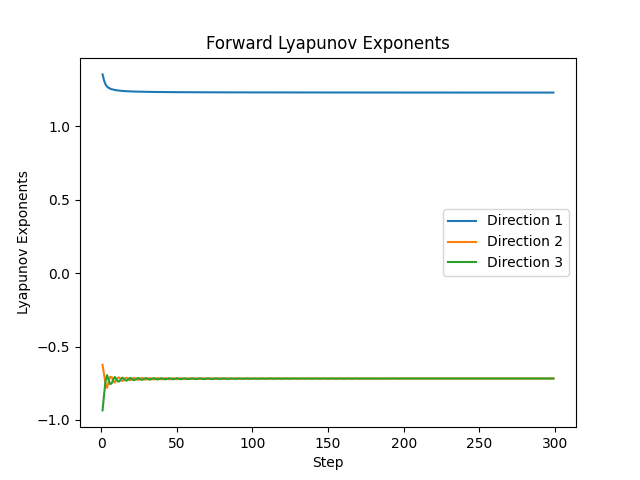
\includegraphics[width=0.7\textwidth]{figures/lyapunov_exponents_forward.png}
  \caption{正向传播收敛情况}
  \label{fig:example}
\end{figure}

由于不考虑输入的影响,反向的李雅普诺夫指数与正向相同:

\begin{figure}[htbp]
  \centering
  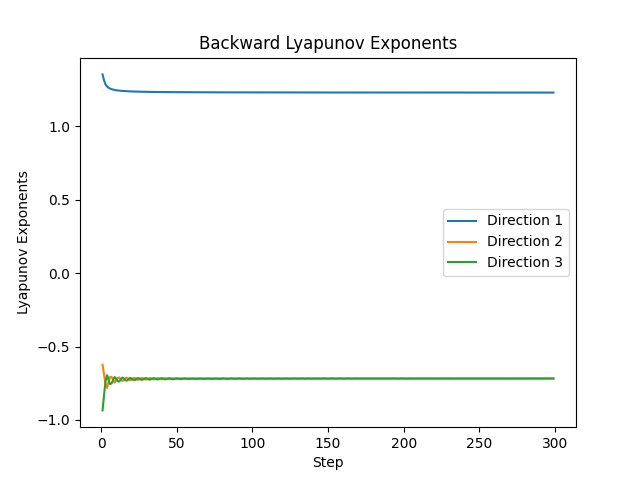
\includegraphics[width=0.7\textwidth]{figures/lyapunov_exponents_backward.png}
  \caption{反向传播收敛情况}
  \label{fig:example}
\end{figure}

在上面的算法中,我们取 $T=300$,运行程序。

实验结果显示,隐藏层的 3 个李雅普诺夫指数分别为:
\begin{equation}
  1.22852421\quad-0.71748841\quad-0.71789691
\end{equation}

根据运行结果显示,正向传播和反向传播的李雅普诺夫指数各自有一个大于 0,两个小于 0,其最大李雅普诺夫指数大于 0,从动力系统的角度分析,其最大李雅普诺夫指数大于 0,表明正向传播和反向传播的梯度不稳定,步数增多可能会导致梯度爆炸。

\subsubsection{运行结果 - 有输入情形}

下面我们进一步验证了有输入情形下的李雅普诺夫谱。我们将输入序列 $\{x_t\}_{t=1}^T$ 设置为随机生成的序列(numpy 的随机数种子设置为 42),以观察李雅普诺夫指数的变化。

运行 300 个时间步后得到的李雅普诺夫指数分别为:

\begin{enumerate}
  \item 正向:
  \begin{equation}
    0.00887475\quad-0.00384957\quad-0.00613681
  \end{equation}
  \item 反向:
  \begin{equation}
    0.00351433\quad-0.0024369\quad-0.00389064
  \end{equation}
\end{enumerate}

正向传播的 300 步的收敛过程如下图所示:

\begin{figure}[htbp]
  \centering
  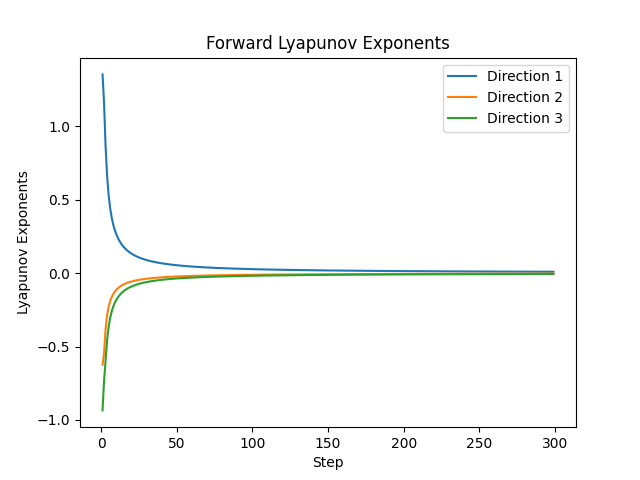
\includegraphics[width=0.7\textwidth]{figures/lyapunov_exponents_forward_with_input.png}
  \caption{有输入情形下的李雅普诺夫指数}
  \label{fig:example}
\end{figure}

反向传播的收敛过程与正向传播类似,且由于李雅普诺夫指数均十分接近 0,图像趋势没有太大区别。同时可以看到,随着 $T$ 的增加,正向和反向传播的李雅普诺夫指数均收敛,这表明前述算法对与一般情形的 RNN 同样有效。

经过对比,加入随机输入因素的前后有如下区别:

\begin{enumerate}
  \item 不考虑输入时,正反的李雅普诺夫谱数值相同,但有输入时,尽管两个李雅普诺夫谱均更接近 0,但二者不再相同。
  \item 加入随机输入后李雅普诺夫指数的绝对值变小,本文暂未找到明确的理论解释。
  \item 加入随机输入后李雅普诺夫指数随 $T$ 的收敛速度更快,对此同样暂没有明确的解释。
\end{enumerate}

虽然有种种不同,但下一节将验证,中间向量的对偶性依旧成立。

\subsection{对偶性的验证}\label{sec:duality}

对偶性的验证用到 \ref{sec:rnn_training} 中记录的中间向量,由算法 \ref{alg:lyapunov} 的原理,它们可以在计算李雅普诺夫谱的同时得到。将这些中间向量输出到日志文件中,然后读取并计算它们的内积,以验证对偶性。

下图形象展示了正向和反向传播的中间向量的内积,横轴表示时间步,可以发现,除去最边缘的极少数时间步,内积图像为一条直线,这表明正向和反向传播的中间向量的内积是一个常数,三条线的纵坐标即为三个方向对应的内积值。

\begin{figure}[htbp]
  \centering
  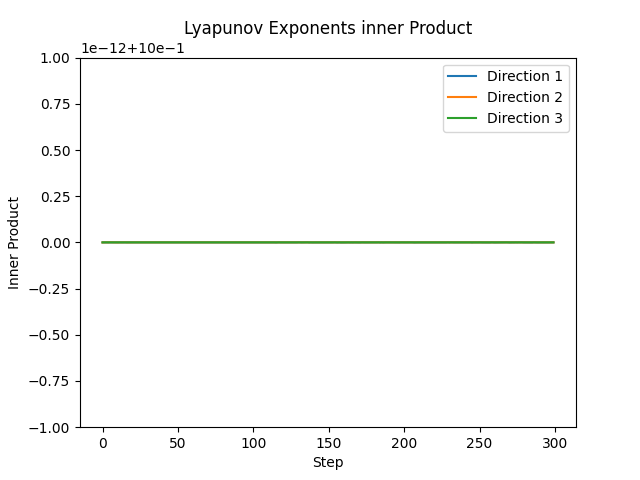
\includegraphics[width=0.7\textwidth]{figures/lyapunov_exponents_inner_product.png}
  \caption{无输入情形下的中间向量 $q_{ij}$ 内积}
  \label{fig:inner_product}
\end{figure}

由此我们便验证了正向传播和反向传播的中间向量 $q_{ij}$ 的有对偶性(不但内积固定,而且三个方向内积相同),但由于提前约定了输入为 0,仅能代表特殊情况,我们还需要进一步验证有输入情形下的对偶性。

使用相同方法,有输入时的中间向量内积如下图所示:

\begin{figure}[htbp]
  \centering
  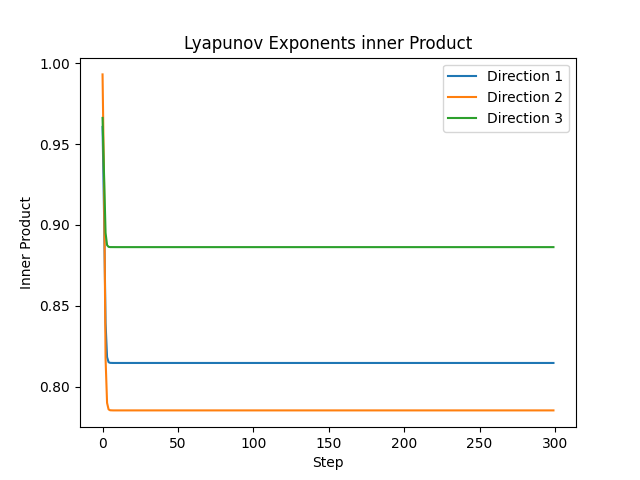
\includegraphics[width=0.7\textwidth]{figures/lyapunov_exponents_inner_product_with_input.png}
  \caption{有输入情形下的中间向量 $q_{ij}$ 内积}
  \label{fig:inner_product_with_input}
\end{figure}

有输入的情形下正反两边的李雅普诺夫谱不再完全相同,但对偶性得到了保留,说明该性质与输入无关,是神经网络本身的特性,由其结构决定。

\section{结论}

本章深入探讨了不稳定神经网络的李雅普诺夫谱和中间向量的对偶性。通过详细的理论分析和实验验证,我们发现李雅普诺夫谱能够有效地揭示神经网络的动态特性,为网络的设计和优化提供了重要的理论支持,值得在未来的研究中进一步应用,此外,对偶性的验证也为神经网络的理论研究提供了新的视角,固定的内积值对于神经网络是否具有更多数学意义,值得进一步探讨。